\chapter{Implementation: Initial detection}
\label{initialdetection}

\begin{figure}[H]
    \begin{center}
        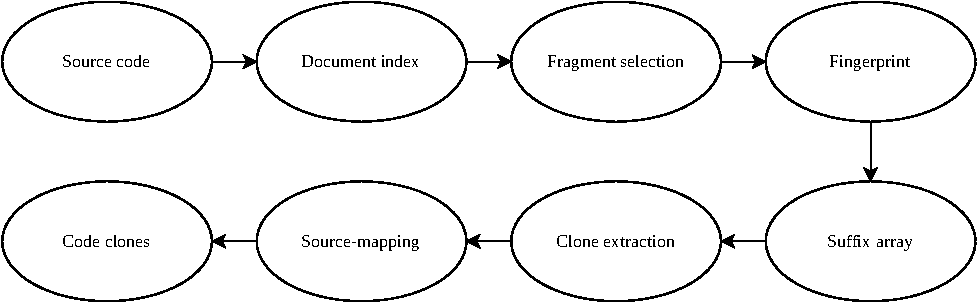
\includegraphics[width=0.8\textwidth]{figures/phases/phases_all.drawio.pdf}
    \end{center}
    \caption{Phases of the detection algorithm}
    \label{fig:allphases}
\end{figure}

This chapter discusses the detection module of CCDetect-LSP and how the initial detection
algorithm finds code clones. It consists of the detection algorithm which takes the
document index as input, and outputs a list of code clones. The initial input to the
algorithm will be the raw source code of each document in the index, in text format.
Figure \ref{fig:allphases} shows all the phases of the detection algorithm and in each
section a figure will be shown to illustrate which part of the pipeline is currently being
discussed. The previous chapter has already detailed the first two phases, how a document
index is built for each file of the source code.

The algorithm of CCDetect-LSP detects syntactical type-1 code clones, based on a token
threshold. Clones detected are therefore snippets of source-code which has at least $N$
equal tokens, where $N$ is a configurable parameter. There are also two types of clones
which are filtered:

\begin{itemize}
    \item Clones which are completely contained within another larger clone are filtered.
    \item Clones cannot extend past the end of a fragment.
\end{itemize}


In broad strokes, the algorithm first selects the relevant parts of source code to detect
code clones in (fragment selection), then transforms the selected fragments into a smaller
representation (fingerprinting). For the matching, an extended suffix array for the
fingerprint is constructed, where the LCP array is used to find long matching instances of
source code. Finally, clones are filtered and aggregated into clone classes before they
are source-mapped back to the original source-code locations, which the LSP server can
send to the IDE in the form of diagnostics.

The decision to go with suffix arrays were based on the fact that suffix arrays use less
memory than the traditional suffix tree approach, which is important in an IDE scenario.
We also wanted to explore dynamic suffix arrays to determine if it could be a better
approach to clone detection performance wise as well, as we are not aware of any work
which compares a dynamic suffix tree with a dynamic suffix array.

\section{Fragment selection}

\begin{figure}[H]
    \begin{center}
        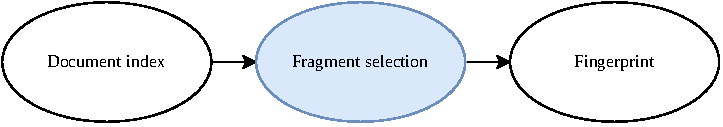
\includegraphics[width=0.8\textwidth]{figures/phases/phases_fragmentselection.drawio.pdf}
    \end{center}
\end{figure}

The first phase of the algorithm involves extracting the relevant fragments of source code
which should be considered for detection. A fragment in this case is considered as a
section of abstract syntax, meaning that a particular type of node in the AST and the
tokens it encompasses should be extracted. Since the algorithm is language agnostic, it is
not feasible to have a single algorithm for fragment extraction or to define a separate
fragment extraction algorithm for every possible language. Therefore, a parser generator
tool is used, which can generate the code for parsing any programming language given a
grammar. We use Tree-sitter, a parser generator with incremental parsing capabilities, as
well as a query language for finding any type of node in the AST~\cite{treesitter}.
Tree-sitter queries are flexible queries to select specific nodes or subtrees. For
example, in Java it would be natural to consider only methods. The Tree-sitter query for
selecting only the method nodes in a Java programs AST would be:

\begin{equation}
    (\mathrm{method\_declaration\ } \text{@method})
\end{equation}

This Tree-sitter query selects the node with type \verb|method_declaration| and
``captures'' it with the \verb|@method| name, so that it can be further processed by the
program. Readers interested in the details of the query system are referred to the
Tree-sitter documentation~\cite{treesitter}.

Using a tree-sitter query, the algorithm parses the program into an AST and queries the
tree for a list of all nodes which matches the query. For each node, all the tokens in the
subtree of the node are extracted and sent to the next phase.

Implementing something similar for another parser/AST could be as simple as traversing the
tree until a node of a specific type is found, using the visitor
pattern~\cite[366]{GangOfFour}.


\section{Fingerprinting}

\begin{figure}[H]
    \begin{center}
        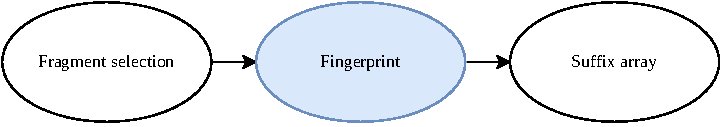
\includegraphics[width=0.8\textwidth]{figures/phases/phases_fingerprint.drawio.pdf}
    \end{center}
\end{figure}

\newsavebox{\firstlisting}
\begin{lrbox}{\firstlisting}
\begin{lstlisting}
public class Math() {
    public int multiplyByTwo(int param) {
        return param * 2;
    }

    public int addTwo(int param) {
        return param + 2;
    }
}
\end{lstlisting}
\end{lrbox}
\begin{figure}[htp]
	\begin{center}
        \subfloat[Source-code] {
            \usebox{\firstlisting}
        }
        \hspace{1cm}
        \subfloat[Fingerprint mapping] {
            \begin{tabular}{l | l}
                Token & Fingerprint \\
			    \hline
                public & 2 \\
                int & 3 \\
                multiplyByTwo & 4 \\
                ( & 5 \\
                param & 6 \\
                ) & 7 \\
                \{ & 8 \\
                return & 9 \\
                * & 10 \\
                2 & 11 \\
                ; & 12 \\
                \} & 13 \\
                addTwo & 14 \\
                + & 15 \\
            \end{tabular}
        }

        \vspace{0.5cm}
        \subfloat[Fingerprint, terminals underlined] {
            [ 2, 3, 4, 5, 3, 6, 7, 8, 9, 6, 10, 11, \underline{1}, 2, 3, 14, 5, 3, 6, 7,
            8, 9, 6, 15, 11, \underline{1}, \underline{0} ]
        }
	\end{center}
	\caption{Example fingerprint of Java source-code}
	\label{fig:fingerprint}
\end{figure}

The next phase of the algorithm is to transform the extracted tokens into a
representation which is less computationally heavy for the matching algorithm. The goal is
to reduce the total size of the input which needs to be processed.

Since the algorithm that is used for matching is based on a suffix array, the
representation should be in a format similar to a string, which is the standard input to a
suffix array construction algorithm. However, it is not strictly necessary to use strings.
The essential property of the input array is that we have a sizeable alphabet where each
element is comparable. We will use an array of integers instead of a string as it has a
large alphabet in most programming languages.

The algorithm utilizes fingerprinting in order to reduce the size of the representation.
Fingerprinting is a technique which involves taking some part of the input and mapping it
to a smaller bit string, which uniquely identifiers that part. In this case, the algorithm
takes each token of the source-code, and maps it to the bit string of an integer. Each
unique token value is mapped to unique integer values. The algorithm keeps a counter,
which is used to fingerprint a token value whenever a new unique token is found. The
algorithm also stores a map from the token value, to the fingerprint value, which is used
to map multiple occurrences of the same token value to the same fingerprint value. Figure
\ref{fig:fingerprint} shows how a sample Java program would be fingerprinted. The
fingerprint mapping initializes its counter at 2 to make space for some terminating
characters. Each fragment is terminated by a $1$ and the fingerprint is ultimately
terminated by a $0$. Having these values in the fingerprint will be useful for the
matching algorithm where the suffix array is constructed and utilized for detection. The
fingerprint of each fragment is stored in the relevant document object.

\section{Suffix array construction}

\begin{figure}[H]
    \begin{center}
        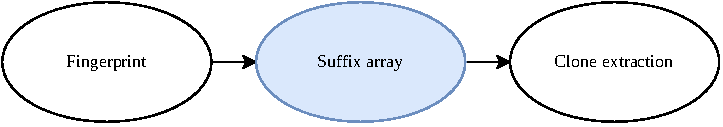
\includegraphics[width=0.8\textwidth]{figures/phases/phases_suffix.drawio.pdf}
    \end{center}
\end{figure}

The next step is to input the fingerprint into a suffix array construction algorithm
(SACA), so that the suffix array can be used to find repeating sequences. Recall that the
suffix array of a string sorts all the suffixes of the string, as discussed in
\cref{prelimalgos}. This makes it simple to find similar regions of text, since similar
suffixes will be next to each other in the suffix array. All the fingerprints which are
stored in each document object will now be concatenated to be stored in a single integer
array (with terminators after each fragment), which the suffix array (SA), inverse suffix
array (ISA) and longest-common prefix array (LCP) is computed from.

We have utilized a straight-forward implementation of the ``Induced sorting
variable-length LMS-substrings'' algorithm~\cite{LinearTimeSuffixArraySAIS} which computes
a suffix array in linear time. The following section will give high-level overview of how
the algorithm works. 

The algorithm will be assumed to have a string as its input, as this is most common for
suffix arrays, and working with strings can be more clear to the reader when considering
suffixes. The algorithm is still applicable to our fingerprint, since an array of integers
will work similarly to a string when given as input.

The ``Induced sorting variable-length LMS-substrings'' algorithm (often abbreviated SA-IS)
is an algorithm that works by divide and conquering the suffix array and inducing how to
sort the suffixes of the string $S$ from a smaller string, $S_1$. $S_1$ consists of the
``building blocks'' of $S$ and will make it simple to compute the rest of the suffix array
of $S$. First, we will introduce some definitions and theorems used for the algorithm.
Input to the algorithm is a string $S$ with length $n$. Let $\mathrm{suffix}(S, i)$ be the
suffix in S starting at position i.

\begin{definition}[L-type and S-type suffixes] A suffix starting at position $i$ in a
    string $S$ is considered to be L-type if it is lexicographically larger than the next
    suffix at position $i + 1$. Meaning that $\mathrm{suffix}(S, i) > \mathrm{suffix}(S,
    i+1)$. Conversely, a suffix is considered to be S-type if $\mathrm{suffix}(S, i) <
    \mathrm{suffix}(S, i+1)$. The sentinel suffix (\$) of $S$ is always S-type.
\end{definition}



\begin{figure}[t]
    \begin{center}
	$$
        \ArrayAccess{\Var{types}}{\Var{n}} = S
	$$
	$$
        \sum^{n - 1}_{i = 0}\ArrayAccess{\Var{types}}{\Var{i}} =
        \begin{cases}
            S & \textrm{if\ } \ArrayAccess{\Var{S}}{\Var{i}} < \ArrayAccess{\Var{S}}{\Var{i + 1}} \\
            L & \textrm{if\ } \ArrayAccess{\Var{S}}{\Var{i}} > \ArrayAccess{\Var{S}}{\Var{i + 1}} \\
            \ArrayAccess{\Var{types}}{\Var{i + 1}} & \textrm{if\ } \ArrayAccess{\Var{S}}{\Var{i}} = \ArrayAccess{\Var{S}}{\Var{i + 1}} 
        \end{cases}
	$$

	\caption{Suffix type recurrence}
	\label{eq:suffixtypesrecurrence}
    \end{center}
\end{figure}

\begin{table}[t]
    \begin{center}
        \begin{tabular}[c]{l l l l l l l}
            B & A & N & A & N & A & \$ \\ 
            L & \underline{S} & L & \underline{S} & L & L & \underline{S} \\ 
            0 & 1 & 2 & 3 & 4 & 5 & 6 \\ 
        \end{tabular}
    \end{center}
    \caption{Suffix types of S = BANANA\$, LMS characters underlined}
    \label{tab:suffixtypesbanana}
\end{table}


\begin{table}[t]
    \begin{center}
        \begin{tabular}[c]{r|cccc}
            Buckets & \$ & A & B & N\\
            Initial & \{ -1 \} & \{ -1, -1, -1 \} & \{ -1 \} & \{ -1, -1 \}\\
            Slot LMS & \{  6 \} & \{ -1,  3,  1 \} & \{ -1 \} & \{ -1, -1 \}\\
            Slot L-type & \{  6 \} & \{  5,  3,  1 \} & \{  0 \} & \{  4,  2 \}\\
            Slot S-type & \{  6 \} & \{  5,  3,  1 \} & \{  0 \} & \{  4,  2 \}\\
        \end{tabular}

        \vspace{0.5cm}
        \begin{tabular}[c]{r|c|c}
                    & \$ & 0 \\
            Mapping & ANA\$ & 1 \\
                    & ANA & 2 \\
        \end{tabular}

        \vspace{0.5cm}

        \begin{tabular}[c]{l|c}
                    $S_1$ & $210$ \\
                    SA of $S_1$ & $[2, 1, 0]$ \\
                    Sorted LMS-substrings & $[6, 3, 1]$ \\
        \end{tabular}

    \end{center}
    \caption{Building $S_1$ and sorting LMS-substrings of S = BANANA\$}
    \label{tab:bucketinglms}
\end{table}


Note that two suffixes in the same string cannot be lexicographically equal, therefore all
cases are handled by this definition. Determining the type of each suffix can be done in
$O(n)$ time by scanning $S$ from right-to-left and observing the following properties:
$\mathrm{suffix}(S, i)$ is L-type if $\ArrayAccess{S}{i} > \ArrayAccess{S}{i + 1}$.
Similarly, $\mathrm{suffix}(S, i)$ is S-type if $\ArrayAccess{S}{i} < \ArrayAccess{S}{i +
1}$. If $\ArrayAccess{S}{i} = \ArrayAccess{S}{i + 1}$, then $\mathrm{suffix}(S, i)$ has
the same type as $\mathrm{suffix}(S, i + 1)$. This is true because if the first character
of the current suffix is not equal to first character of the next suffix, we already know
the type based on the first character. If the first character is equal, we have
effectively transformed the problem to finding the type of the next suffix, since we are
now comparing the second character of the current suffix, with the second character of the
second suffix. Since we have already computed the type of the next suffix, we can reuse
the value. Figure \ref{eq:suffixtypesrecurrence} shows a recurrence which determines the
type of each suffix in a string in $O(n)$ time and table \ref{tab:suffixtypesbanana} shows
an example.

\begin{definition}[LMS character]

    An LMS (Left-most S-type) character in a string $S$ is a position $i$ in $S$ such that
    $S[i]$ is S-type and $S[i-1]$ is L-type. An LMS-suffix is a suffix in $S$ which begins
    with an LMS character. The final character of $S$ (the sentinel) is always an LMS
    character and the first character is never an LMS character.

\end{definition}

\begin{definition}[LMS-substring]

    An LMS-substring in a string $S$ is a substring $S[i..j]$ in $S$ such that $i \neq j$,
    $S[i]$ and $[j]$ are LMS characters and there are no other LMS characters between. The
    sentinel character is also an LMS-substring and is the only LMS-substring of length
    $\leq 3$

\end{definition}

LMS-substrings form "basic-blocks" in the string $S$. Each LMS-substring is mostly
lexicographically decreasing or increasing, which is easier to sort. Table
\ref{tab:bucketinglms} shows that in the string BANANA\$ there are 3 S-type suffixes
and all of them form LMS-substrings (ANA, ANA\$, \$). Using this notion, we can sort all
suffixes recursively using the following theorems:

\begin{theorem}

    Given sorted LMS-suffixes of $S$, the rest of the suffix array can be induced in linear
    time. 

\end{theorem}

\begin{theorem}
    There are at most $n / 2$ LMS-substrings in a string $S$ of length n.
\end{theorem}

These theorems are proven in the original paper, we will now use these theorems to show
how we can compute the suffix array in linear time. Table \ref{tab:bucketinglms} shows a
running example of the algorithm. We can construct a smaller string $S_1$ by first sorting
the LMS-substrings. Sorting LMS-substrings can be done by first bucket-sorting each
LMS-substring by its first character. The buckets are implemented as arrays and each
LMS-substring is inserted at the end of the correct bucket. Afterwards, L-type suffixes
are bucketed by iterating over the buckets, and for each suffix in the bucket, insert the
suffix to the left, if it is L-type. Meaning that if we encounter the suffix at position
6, the suffix at position 5 is bucketed if it is L-type. Finally, S-type suffixes are
bucketed similarly in the same fashion, but the buckets are scanned from right-to-left and
suffixes are inserted at the end of the bucket. This final step could possibly change the
ordering of the LMS-substrings.

After sorting, each equal LMS-substring is given a unique increasing integer value. Two
LMS-substrings are considered equal if they are equal in terms of length, characters and
types. $S_1$ is now built by mapping each LMS-substring to its unique value, and
concatenating them in the original ordering. $S_1$ is now a smaller case which is used in
the recursion. The string is at most $n / 2$ in size, meaning there will be at most
$\log_2(n)$ recursive calls. The recursive call will return the suffix array of the $S_1$.
Nong et al. proves a theorem which shows that sorting $S_1$ is
equivalent to sorting the LMS suffixes of $S$. Therefore, the suffix array of $S_1$ can be
mapped to the LMS suffixes of $S$~\cite{LinearTimeSuffixArraySAIS}.

The base-case of the recursion is when the suffix array can be computed simply by
bucketing each suffix, which happens when every suffix of the string starts with a unique
character. 

Table \ref{tab:bucketinglms} shows how the LMS-substrings are bucketed and how $S_1$ is
constructed. We see that the final buckets are actually equal to the final SA which we are
trying to compute. This is because the LMS-substrings are already sorted in reverse order,
which is not true for any arbitrary input. $S_1$ consists of only unique characters,
therefore the suffix array of $S_1$ is computed by simply bucketing each suffix and
returning the array.

When the recursive call returns, the SA of $S_1$ is used to determine the order which the
LMS-suffixes should be slotted into the bigger SA. By scanning the smaller SA and mapping
those indices back to the indices of the original LMS-substrings, we get a sorted ordering
of the LMS-suffixes. We then scan the sorted LMS-suffixes from right-to-left and slot each
LMS-suffix at the end of its bucket, the rest of the L-type and S-type suffixes will be
slotted correctly afterwards. For BANANA\$ this will be the exact same process as in table
\ref{tab:bucketinglms}, since the LMS-substrings were already inserted in reverse
ordering.

There will be $O(\log_2(n))$ recursive call, where each recursive call takes $O(n)$ time,
with $n$ halving in each call. Therefore, the recurrence will have the complexity of:

\begin{gather*}
    T(n) =
\begin{cases}
    O(n) & \text{if base-case.} \\
    T(n / 2) + O(n)
\end{cases}
= O(n)
\end{gather*}

\subsection*{Building ISA and LCP arrays}

Computing the ISA after constructing the SA is simple. Since the ISA is simply the inverse
of SA, it can be constructed in linear time with a single loop as seen in Algorithm
\ref{alg:isa}.

\begin{algorithm}[t]
  \SetAlgoLined\DontPrintSemicolon
    \algo{\ComputeISA{SA}}{
    $\Var{n} \gets \Len{$\Var{SA}$}$ \\
    $\Var{ISA} \gets \mathrm{array\ of\ size\ n}$

        \For{$\Var{i} \From 0 \To \Var{n}$}{
            $\ISA{\SA{i}} \gets \Var{i}$
        }

        \Return $\Var{ISA}$
    }

  \vspace{0.5cm}
  \caption{Compute ISA from SA}
  \label{alg:isa}
\end{algorithm}


Computing the LCP in linear time is more complicated and requires some insight about which
order to insert LCP values. We will also add one extra restriction to the LCP values,
being that the LCP values cannot match past a $1$, which were the terminal value between
fragments. This restriction will be useful when we want to extract clones using the LCP
array. The algorithm to compute the LCP is shown in Algorithm \ref{alg:lcp}. The intuition
for this algorithm is that if a suffix at position $i$ has an LCP value $l$ describing the
common-prefix between it and some other suffix at position $j$, then the LCP value of the
suffix at position $i + 1$ is at least $l - 1$, since there exists suffixes at position $i
+ 1$ and $j + 1$ which shares at minimum $l$ characters, except for the first character
which is cut off. Therefore, they share at least $l - 1$ characters, and the algorithm can
start comparing the characters at that offset.

\begin{algorithm}[t]
  \SetAlgoLined\DontPrintSemicolon
    \algo{\ComputeLCP{S, SA, ISA}}{
        $\Var{n} \gets \Len{$\Var{SA}$}$

        $\Var{LCP} \gets \mathrm{array\ of\ size\ n}$

        $\Var{lcpLen} \gets 0$

        \For{$\Var{i} \From 0 \To \Var{n} - 1$}{
            $\Var{r} \gets \ISA{i}$

            $\Var{prevSuffix} \gets \SA{\Var{r} - 1}$

            \While{$\ArrayAccess{\Var{S}}{\Var{i} + \Var{lcpLen}} =
            \ArrayAccess{S}{\Var{prevSuffix} + \Var{lcpLen}} \And \ArrayAccess{S}{\Var{i} +
        \Var{lcpLen}} \neq 1$}{
                $\Var{lcpLen} \gets \Var{lcpLen} + 1$
            }

            $\LCP{\Var{r}} \gets \Var{lcpLen}$

            $\Var{lcpLen} \gets \Max{$0, \Var{lcpLen} - 1$}$
        }

        \Return ISA
    }

  \vspace{0.5cm}
  \caption{Compute LCP from input string S, SA, and ISA}
  \label{alg:lcp}
\end{algorithm}

\begin{table}[t]
    \begin{center}
        \begin{tabular}[c]{c|cccccc|c}
            Index & \multicolumn{6}{c}{Suffix} & Minimum LCP \\
            \hline
            1 & A & N & A & N & A & \$ & 0 \\ 
            3 & A & N & A & \$ &  &  & 0\\ 
            2 & N & A & N & A & \$ & & 2 \\ 
            4 & N & A & \$ & & &  & 2\\ 

        \end{tabular}
    \end{center}
    \caption{Minimum common LCP values between suffixes for S = BANANA\$}
    \label{tab:}
\end{table}

Now that we have computed the extended suffix array in linear time, we are ready to detect
clones in our code base using this data structure.

\section{Clone extraction}

\begin{figure}[H]
    \begin{center}
        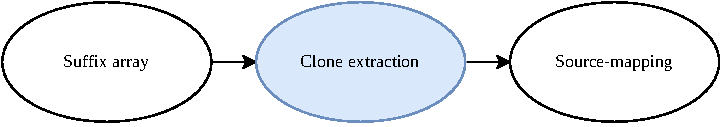
\includegraphics[width=0.8\textwidth]{figures/phases/phases_cloneextraction.drawio.pdf}
    \end{center}
\end{figure}

With the extended suffix array computed, we can now consider which substrings (prefixes of
suffixes) we want to extract as potential code clones. In this phase the indices of the
fingerprint which we consider to be code clones are extracted, which will be mapped back
to the original source code in the next phase.

\begin{algorithm}[t]
  \SetAlgoLined\DontPrintSemicolon
    \algo{\SimpleCloneExtraction{S, ISA, LCP}}{
        $n \gets \Access{S}{len}$ \;
        $\Var{clones} \gets \Var{list}$ \;


        \For{$i \From 0 \To n - 1$}{
            \If{$\ISA{\Var{i}} = 0$}{
                \Continue \;
            } \;

            \If{$\LCP{\ISA{\Var{i}}} \geq \text{THRESHOLD}$}{
                $\Insert{$\Var{clones}, \Var{i}$}$ \Comment{Adds i to the clone-list}
            }
        }

        \Return clones
    }

  \vspace{0.5cm}
  \caption{Extract clones indices in a string $S$}
  \label{alg:simplecloneextraction}
\end{algorithm}

\begin{algorithm}[t]
  \SetAlgoLined\DontPrintSemicolon
    \algo{\CloneExtraction{S, ISA, LCP}}{
        $\Var{n} \gets \Access{\Var{S}}{\Var{len}}$ \;
        $\Var{clones} \gets \textrm{empty\ list}$ \;


        \For{$\Var{i} \From 0 \To \Var{n} - 1$}{
            \If{$\ArrayAccess{\Var{ISA}}{i} = 0$}{
                \Continue \;
            } \;

            \If{$\ArrayAccess{\Var{LCP}}{\ArrayAccess{\Var{ISA}}{\Var{i}}}  \geq \Var{THRESHOLD}$}{
                $\Insert{$\Var{clones}, \Var{i}$}$ \tcp{Adds i to the clone-list} \;


                \While{$\Var{i} + 1 < \Var{n} \And
                \ArrayAccess{\Var{LCP}}{\ArrayAccess{\Var{ISA}}{\Var{i} + 1}} <
            \ArrayAccess{\Var{LCP}}{\ArrayAccess{\Var{ISA}}{\Var{i}}}$}{
                    $\Var{i} \gets \Var{i} + 1$
                }

            }
        }

        \Return $\Var{clones}$
    }

  \vspace{0.5cm}
  \caption{Extract clones indices in a string $S$, ignoring contained clones}
  \label{alg:cloneextraction}
\end{algorithm}

A straightforward solution is to extract every suffix which has an LCP value which is
greater than the token threshold. The algorithm is a loop over $S$, using ISA to find the
corresponding LCP value. This finds the clone indices, as shown in Algorithm
\ref{alg:simplecloneextraction}.


However, this algorithm will return a lot of contained clones. A contained clone is a
clone where all the tokens of the clone is a part of another, larger clone. The algorithm
will give a lot of contained clones, for example in the case where there is a suffix with
an LCP value of $100$, the next suffix will have the LCP value of at least $99$ and likely
matches with the same code clone as the previous suffix, but with an offset of 1 token.
For any large code clone, there will therefore be many smaller clones which are completely
contained within it, but these clones are also likely to match with another clone which is
also contained within the larger clones match. Since the code clones point at mostly the
same area, the contained clones are not very useful, and should not be considered. We
extend our clone extraction algorithm to account for this, by using the following theorem:

\begin{theorem} 

    The LCP of a suffix at position $i$ is completely contained in the LCP of the previous
    suffix at position $i - 1$ if the LCP value of the suffix at position $i - 1$ is
    greater than the LCP value of the suffix at position $i$. Meaning $\LCP{\ISA{\Var{i}}}
    < \LCP{\ISA{\Var{i} - 1}}$.


\end{theorem}


Algorithm \ref{alg:cloneextraction} adds a while-loop to the clone extraction algorithm
which skips over suffixes which are contained according to the theorem. Note that this
algorithm doesn't disallow contained clones entirely, but any clone which is a shorter
version of another clone pointing to the same match, will be filtered. Also note that
overlapping clones, meaning two clones which share tokens, but where neither contains the
other, will not be filtered.

At the end of this phase we now have a list of indices in the fingerprint which is
considered to be code clones.

\section{Source-mapping}

\begin{figure}[H]
    \begin{center}
        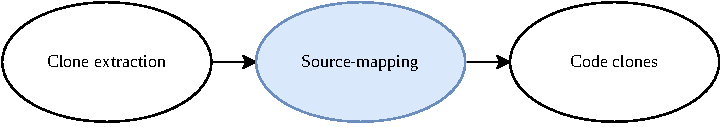
\includegraphics[width=0.8\textwidth]{figures/phases/phases_sourcemap.drawio.pdf}
    \end{center}
\end{figure}

With the clone indices in the fingerprint computed, we are almost finished. The final step
is to map the clone indices back to the original source code. In order to correctly
identify where a clone is located, we need to know which file the clone is located in, the
range of the source code in that file the code clone covers, and the other matching code
clones.

To accomplish this, each document in the index needs to store the range of each of its
tokens and keep track of which portion of the fingerprint consists of the documents
tokens. This is done by storing two integer variables, each storing the start position and
end position that the document has in the fingerprint. 

\begin{algorithm}[t]
  \SetAlgoLined\DontPrintSemicolon
    \algo{\SourceMap{documents, i}}{
        $\Var{left} \gets 0$ \;
        $\Var{right} \gets \Access{\Var{documents}}{\Var{len}} - 1$ \;\;


        \While{$\Var{left} \leq \Var{right}$}{
            $\Var{mid} \gets (\Var{left} + \Var{right}) / 2$

            \uIf{$\Access{\ArrayAccess{\Var{documents}}{\Var{mid}}}{\Var{end}} < i$}{
                $\Var{left} = \Var{mid} + 1$
            }
            \uElseIf{$\Access{\ArrayAccess{\Var{documents}}{\Var{mid}}}{\Var{start}} > i$}{
                $\Var{right} = \Var{mid} - 1$
            }
            \Else {
                $\Var{D} \gets \ArrayAccess{\Var{documents}}{\Var{mid}}$ \;
                $\Var{range} \gets \ArrayAccess{\Access{\Var{D}}{\Var{ranges}}}{\Var{i} -
                \Access{\Var{D}}{end}}$

                \Return $(\Access{\Var{D}}{\Var{uri}}, \Var{range})$
            }

        }
    }

  \vspace{0.5cm}
  \caption{Get source-map for a position $i$ in the fingerprint}
  \label{alg:sourcemap}
\end{algorithm}

To determine which document a fingerprint position corresponds to, we can perform a binary
search on the list of the documents, which is sorted based on the start position of the
documents fingerprint. The goal is to find the document $D$ where the fingerprint position $i$
is 

$$
\Access{D}{start} \leq i \leq \Access{D}{end}
$$

Once the correct document has been found, we simply have to look up the correct range
which the document stores. The index of this range is $i -
\Access{D}{start}$.

Algorithm \ref{alg:sourcemap} returns the source-map of a given position $i$ in the
fingerprint, which includes the URI for the document and the source code range of the
token at position $i$.

This algorithm only shows how to look up the position of a single token. Since a code
clone is a range between two tokens, we have to look up the position at index $i$
extracted in the previous phase, and the position where the clone ends, which is index $i
+ \text{LCP}[\text{ISA}[i]]$. The range of the code clone is therefore the combination of
the starting range of the first token (at position $i$) and the ending range of the second
token (at position $i + \text{LCP}[\text{ISA}[i]]$):

\subsection*{Aggregating clones}

With this algorithm to get the clone locations, the next step is to make sure that
matching code clones are collected into buckets of clone classes. Remember that the LCP
array only gives us the longest match between two suffixes, but it is naturally possible
to have more than two clones of the same code snippet. This case happens when multiple
consecutive indices in the SA are considered to be clones. Since we only look for type-1
clones, the transitivity property holds, meaning that if

$$
SA[i] \xrightarrow{clone} SA[i+1] \xrightarrow{clone} SA[i + 2]
$$

then clones at position $SA[i]$, $SA[i+1]$ and $SA[i + 2]$ are all clones of each other.
This should be achieved by making sure that every new clone-pair discovered adds
previously detected clones to their clone sets, and previously discovered clones also add
new clones to theirs. Figure \ref{fig:cloneaggregation} shows how a new match is found in
two previously disjoint clone classes, and the resulting aggregated clone class.

This is achieved in algorithm \ref{alg:buildclonemap} where we build a clone-map, where
the key is the index that a clone starts at in the fingerprint. For each clone index $i$
which was extracted in the last phase, we get the corresponding match index $j$
($\text{SA}[\text{ISA[i]} - 1]$), and for both $i$ and $j$ we look in the clone-map if
there already is a clone at that position, or a new clone object is created and put in the
map. Then, in order to aggregate the previously discovered clones and the new clone
together, the set of matching clones is unioned between the two clones. In this way, all
the previous existing clones of $i$ is added as a clone in $j$ and vice versa. Every clone
in the two clone classes will then receive the same set of code clones. The
\verb|UnionCloneClass| function unions all the clone sets in both clone classes and then
adds a match from all clones in one clone class to all clones in the other.

Finally, we have a list of every code clone in the code base, which is then sent to the
LSP module of the tool, which handles the displaying of code clones to the client as
shown in \cref{lspimplementation}.

\begin{figure}[t]
    \begin{center}
        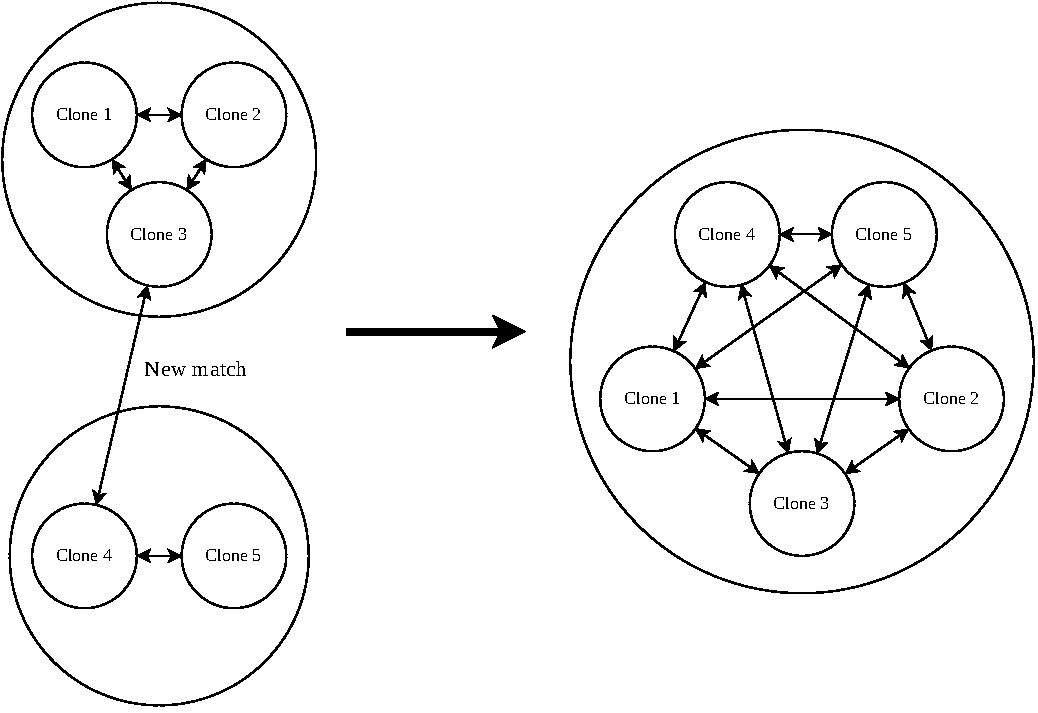
\includegraphics[width=0.95\textwidth]{figures/cloneaggregation.drawio.pdf}
    \end{center}
    \caption{Clone class aggregation when a new match is found}
    \label{fig:cloneaggregation}
\end{figure}

\begin{algorithm}[t]
  \SetAlgoLined\DontPrintSemicolon
    \algo{\GetCloneMap{index, cloneIndices}}{
        $\Var{n} \gets \Access{\Var{cloneIndices}}{\Var{len}}$ \;
        $\Var{cloneMap} \gets \textrm{Empty map with type: } \Var{int} \rightarrow \Var{CodeClone}$ \;\;

        
        \For{$\Var{i} \From 0 \To \Var{n} - 1$}{
            $\Var{firstIndex} \gets \ArrayAccess{\Var{cloneIndices}}{\Var{i}}$ \;
            $\Var{secondIndex} \gets \SA{\ISA{\Var{firstIndex}} - 1}$ \;
            $\Var{size} \gets \LCP{\ISA{\Var{firstIndex}}} - 1$ \;\;


            \Comment{Use SourceMap function to get ranges and documents of clones}
            $\Var{firstRange} \gets \textrm{Get source between firstIndex and
            (firstIndex + size)}$ \;
            $\Var{secondRange} \gets \textrm{Get source between secondIndex and
            (secondIndex + size)}$ \;\;

            $\Var{firstDocument} \gets \Access{\Var{firstRange}}{\Var{document}}$ \;
            $\Var{secondDocument} \gets \Access{\Var{secondRange}}{\Var{document}}$ \;\;
            
            \Comment{Build clone objects if they don't exist}
            \If{$\Var{firstIndex} \NotIn \Var{cloneMap}$}{
                $\Var{firstClone} \gets \New
                \CodeClone{$\Access{\Var{firstDocument}}{\Var{uri}},
                \Var{firstRange}$}$ \;
                $\Put{$\Var{cloneMap}, \Var{firstIndex}, \Var{firstClone}$}$ \Comment{Put
                clone with firstIndex as key}
            }
            \If{$\Var{secondIndex} \NotIn \Var{cloneMap}$}{
                $\Var{secondClone} \gets \New
                \CodeClone{$\Access{\Var{secondDocument}}{\Var{uri}},
                \Var{secondRange}$}$ \;
                $\Put{$\Var{cloneMap}, \Var{i}, \Var{secondClone}$}$ \Comment{Put
                clone with secondIndex as key}
            } \;

            \Comment{Union clone classes}
            \UnionCloneClass{\Get{$\Var{cloneMap}, \Var{firstIndex}$}, \Get{$\Var{cloneMap,
            \Var{secondIndex}}$}} \;
        }
        \Return $\Var{cloneMap}$
    }

  \vspace{0.5cm}
  \caption{Build clone-map given the clone indices in the fingerprint}
  \label{alg:buildclonemap}
\end{algorithm}
